\section{INTRODUCTION}
The importance of sensors in a control loop goes without saying.
% ~\cite{SomeoneIfoundAndThatInoLongerFind}.
Measurement devices, however, can seldom be used \emph{sine die} without being subject to periodic calibration procedures.
Pressure transducers, gas sensors, and thermistors are only a few examples of measuring devices that need to be calibrated periodically for providing 
the user with precise and robust measurements.
Of most importance, calibration procedures may require to move the sensor from the hosting system to specialized laboratories, which are equipped with
the tools for performing the calibration of the measuring device. This paper presents techniques to calibrate 
strain gauges six-axis force-torque sensors \emph{in situ}, i.e. without the need of removing the sensor from the hosting system.
The proposed calibration method is particularly suited for robots with embedded six-axis force-torque sensors installed within limbs~\cite{Fumagalli2012}. 

Calibration of six-axis force-torque sensors  has long attracted the attention of the robotic community~\cite{braun2011}. 
The commonly used model for predicting the force-torque 
from the raw measurements of the sensor is an affine model.
This model is sufficiently accurate 
since these sensors are mechanically designed and mounted so that the strain deformation is (locally) linear with respect to the applied forces and torques.
Then, the calibration of the sensor aims at determining the two components of this model, i.e. a six-by-six matrix and a six element vector.
These two components are usually referred to as the sensor's \emph{calibration matrix} and \emph{offset}, respectively.
In standard operating conditions, relevant changes in the calibration matrix may occur in months.
As a matter of fact, manufacturers such as ATI~\cite{atimanual} and Weiss Robotics~\cite{kms40manual} 
recommend to calibrate force-torque sensors at least once a year.
Preponderant changes in the sensor's offset can occur in hours, however, and this in general requires to estimate the 
offset before using the  sensor.
The offset models the sensitivity of the semiconductor strain gauges with respect to temperature.

\begin{figure}
\vspace{0em}
\centering
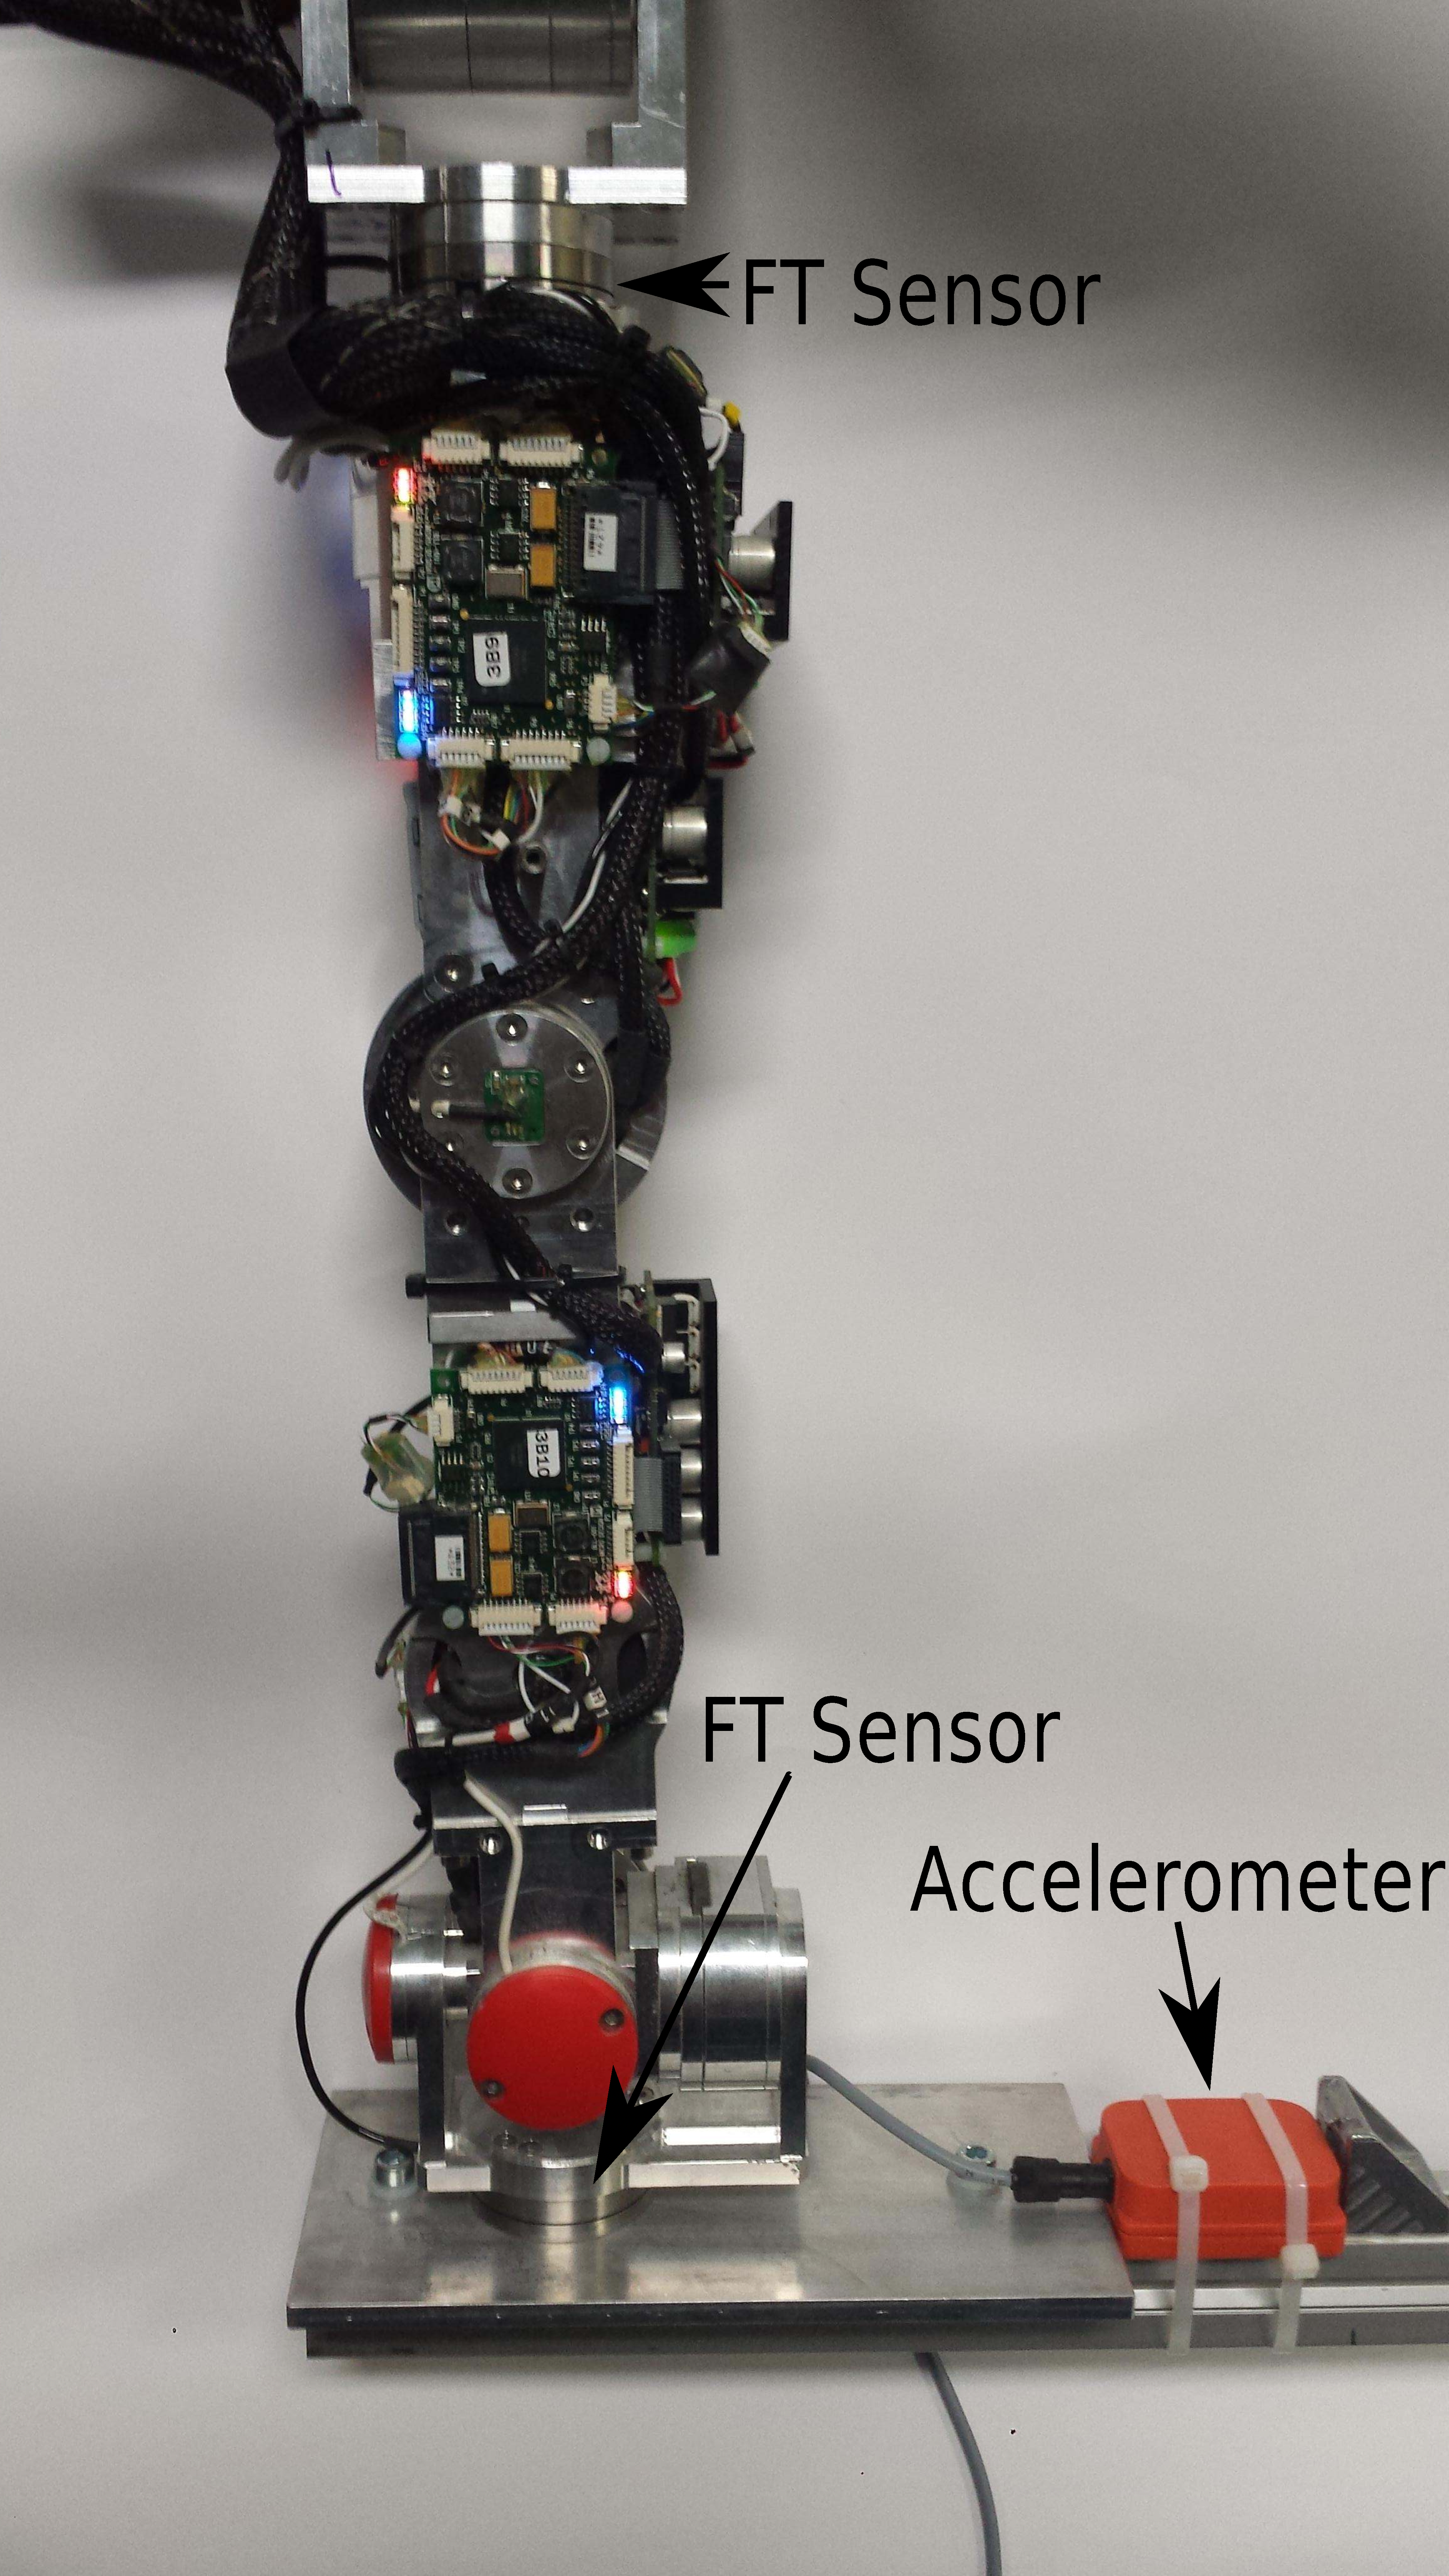
\includegraphics[width=0.225\textwidth]{images/leg.pdf};
\caption{iCub's leg with the two force/torque sensors and an additional accelerometer.}
\label{fig:iCubLeg}
\end{figure} 
Classical techniques for determining the offset of a force-torque sensor exploit the aforementioned affine model between 
the raw measurements and the load attached to the sensor. In particular, if no load is applied to the measuring device, the output of the sensor corresponds to 
the sensor's offset. This offset identification procedure, however, cannot be always performed since it may require to take the hosting system apart
in order to unload the force-torque sensor. Another widely used technique for offset identification is to find two sensor's orientations that induce
equal and opposite loads with respect to the sensor. Then, by summing up the raw measurements associated with these two orientations, one can estimate
the sensor's offset. The main drawback of this technique is that the positioning of the sensor at these opposite configurations may require to move
the hosting system beyond its operating domain.

Assuming a preidentified offset, non-in situ identification of the calibration matrix is classically performed by exerting on  
the sensor a set of force-torques known \emph{a priori}. This usually requires to place 
sample masses at precise relative positions with respect to the sensor. Then, by comparing
the known gravitational force-torque with that measured by the sensor, 
one can apply linear least square techniques to identify the sensor's calibration matrix.
For accurate positioning of the sample masses, the use of robotic positioning devices 
has also been proposed in the specialized 
literature~\cite{uchiyama1991systematic}~\cite{watson1975pedestal}.
%Clearly, the more numerous the sample masses, the smaller the identification error. 

To reduce the number of sample masses,
one can apply constrained forces, e.g. constant norm forces, to the measuring device.
Then these constrains can be exploited during the computations for identifying the calibration matrix~\cite{voyles1997shape}.
To avoid the use of added masses, one can use a supplementary already-calibrated measuring device that measures 
the force-torque exerted on the sensors~\cite{faber2012force}~\cite{oddo2007}.
On one hand, this calibration technique avoids the problem of precise positioning of the added sample masses.
On the other hand, 
the supplementary sensor may not always be available.
All above techniques, however, cannot be performed in situ, thus  being usually time consuming and expensive.


To the best of our knowledge, the first \emph{in situ} calibration method for force-torque sensors was proposed 
in \cite{shimanoroth}. But this method  exploits the topology of a specific kind of manipulators, which are equipped with
joint torque sensors then leveraged during the estimation. 
A recent result~\cite{Gong2013} proposes another \emph{in situ} calibration technique for six-axis force-torque sensors. 
The technical soundness of this work, however, is not clear to us. In fact, we show that a necessary condition for identifying the calibration matrix
is to take measurements for at least three different added masses, and this requirement was not met by the algorithm~\cite{Gong2013}.
Another in situ calibration technique for force-torque sensors can be found in \cite{roozbahani2013novel}.
But the use of supplementary already-calibrated force-torque/pressure sensors impairs this technique for the reasons we have discussed before. 




This paper presents in situ calibration techniques for six-axis force-torque sensors using accelerometer measurements.
The proposed method exploits the geometry induced by the affine model between the raw measurements and the gravitational force-torque applied to the sensor. 
In particular, it relies upon the properties that all gravitational raw measurements belong to a three-dimensional space, and that in this space they form an ellipsoid.
Then, the contribution of this paper is twofold. We first propose a method for estimating the sensor's offset, and then a procedure for identifying
the calibration matrix. The latter is independent from the former, but requires to add sample masses to the rigid body attached to the sensor. Both methods are independent from the inertial characteristics 
of the rigid body attached to the sensor. 
The proposed algorithms are validated on the iCub platform by calibrating
two force-torque sensors embedded in the robot~leg.

The paper is organized as follows. Section~\ref{sec:background} presents the notation used in the paper and the problem statement with the assumptions. 
Section~\ref{method} details the proposed method for the calibration of six-axis force-torque sensors. 
Validations of the approach are presented in Section~\ref{experiments}.
Remarks and perspectives conclude the paper.


